%       INTRO
%       TRANSFORMÉE MULTI-ÉCHELLE
%       HEURISTIQUES D'ADAPTATION
%       ALGORITHMES
%           CALCULS NIVEAU COURANT
%           CALCUL NIVEAU FIN
%       SOURCES D'ERREURS
%       IMPLÉMENTATIONS
%           MÉTHODES CLASSIQUES 
%           SAMURAI

% Ce seuil $\varepsilon$ n'est pas l'unique juge lors la compression, des heuristiques reposant sur la quantité d'information des détails de niveau supérieur
% sont utilisées pour ne pas seuiller systématiquement. L'objectif est en quelque sorte d'anticiper le besoin de détails\footnote{Même si la quantité d'information laisse entendre que 
% certains détails pourraient être ignorés, l'intuition physique pose sont veto et force certains détails à être conservés par précaution, par exemple si un front front d'onde arrive.}.
% La plus connue est l'heuristique d'Ami Harten \cite{harten1994}.

La multi-résolution adaptative (MRA) est une méthode permettant de représenter une fonction selon différentes échelles.
Cet outil mathématique peut être exploité pour réaliser l'adaptation en espace d'une solution physique pour concentrer les efforts computationnels là où ils sont nécessaires. 
Cette approche très efficace pour les problèmes multi-échelles.
L'adaptation dynamique de maillage par MRA est très étudiée par l'équipe du CMAP qui a développé le code Samurai\footnote{\href{https://github.com/hpc-maths/samurai}{https://github.com/hpc-maths/samurai}}
centré sur cette méthode.
\begin{figure}[h]
    \centering
    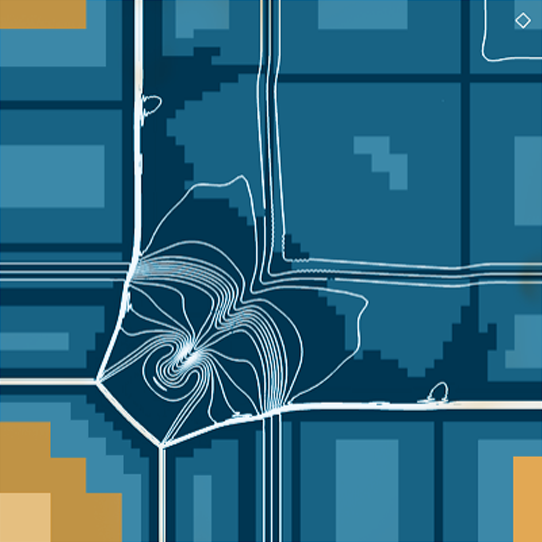
\includegraphics[width=0.5\textwidth]{media/3_/3_/exemple_compression_samurai.png}
    \caption{Exemple de maillage adapté par multirésolution adaptative grâce au logiciel \href{https://github.com/hpc-maths/samurai}{Samurai}.}
    \label{fig:samurai}
\end{figure}
Concrètement cela consiste à augmenter la résolution de la grille de calcul où la solution est complexe et la diminuer où la solution est simple à décrire.
La MRA est donc une méthode de HPC (\textit{high performance computing}) puisqu'elle vise à optimiser l'allocation des ressources de calcul.\par
Cette partie introduit le lecteur à cette méthode en présentant d'abord le concept mathématique de transformée multi-échelle (ou transformée en ondelette). 
Puis il est expliqué comment la transformée multi-échelle permet d'adapter le maillage pour optimiser la charge computationnelle.
Une fois ces prérequis établis, l'algorithme typique de mise en oeuvre de la multi-résolution adaptative est décrit.
Vient enfin une présentation des différentes implémentations de la MRA.
% Enfin l'impact de la multi-résolution sur la qualité des solutions numériques est abordé.

\subsection{La représentation multi-échelle}
    La représentation multi-échelle est la clé de voûte de l'adaptation par AMR.
    Cette partie traite le cas où l'on souhaite obtenir la représentation multi-échelle d'une fonction $u(\cdot) \in L^2([0,1])$, 
    mais cela s'étend sans trop de difficulté au dimensions supérieures.
    La représentation multi-échelle se base une description de l'intervalle $[0,1]$ en grilles dyadiques de résolutions différentes
    et sur deux opérateurs permettant de naviguer d'un niveau de résolution à l'autre : un opérateur de projection et un opérateur de prédiction.
    \subsubsection{Les grilles dyadiques}
        La représentation multi-échelle permet de représenter la solution à différents niveaux de résolution. 
        Ainsi si l'on choisit de représenter la solution entre des niveau de résolution $\overline j > \underline j$, 
        il faut définir pour chaque niveau de résolution $j \in \left\{ \underline j, \dots, \overline j\right\}$ une grille dyadique, c'est à dire une partition de $[0,1]$
        composée de cellules $\left(C^j_k\right)_{k \in \left\{0\dots 2^{j}-1\right\}}$ de tailles $2^{-j}$ où $C^j_k = \left[k\,2^{-j} ,(k+1)2^{-j}\right]$.\par
        Dans le cadre des volumes finis, une fonction $u \in L^2\left(\left[0,1\right]\right)$ est discrétisée
        à un niveau de résolution $j$ en associant la cellule $C^j_k$ à la valeur moyenne de $u(\cdot)$ sur cette cellule :
        \begin{align}
            u^j_k = \frac{1}{2^{j}} \int_{C_j} u(x) \, \mathrm{d}x.
        \end{align}
        \begin{figure}[htbp]
    \centering
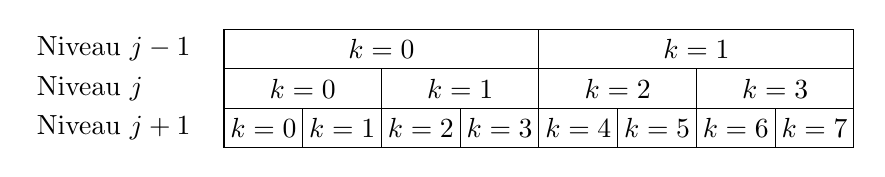
\begin{tikzpicture}


\node[anchor=west] at (-6.5, -.25) {Niveau $j+1$};
\node[anchor=west] at (-6.5, .25) {Niveau $j$};
\node[anchor=west] at (-6.5, .75) {Niveau $j-1$};
% Niveau j-1

\draw (-4,.5) rectangle (0,1);
\draw (0,.5) rectangle (4,1);

    % Niveau j
\draw (-4,0) rectangle (-2,.5);
\draw (-2,0) rectangle (0,.5);
\draw (0,0) rectangle (2,.5);
\draw (2,0) rectangle (4,.5);
%\node at (1,1.75) {$k=2$};

% Niveau j+1

\draw (-4,-.5) rectangle (-3,0);
\draw (-3,-.5) rectangle (-2,0);
\draw (-2,-.5) rectangle (-1,0);
\draw (-1,-.5) rectangle (0,0);
\draw (0,-.5) rectangle (1,0);
\draw (1,-.5) rectangle (2,0);
\draw (2,-.5) rectangle (3,0);
\draw (3,-.5) rectangle (4,0);

% Relations
\node at (-2, .75) {$k=0$};
\node at (+2, .75) {$k=1$};

\node at (-3, .25) {$k=0$};
\node at (-1, .25) {$k=1$};
\node at (+1, .25) {$k=2$};
\node at (+3, .25) {$k=3$};

\node at (-3.5, -.25) {$k=0$};
\node at (-2.5, -.25) {$k=1$};
\node at (-1.5, -.25) {$k=2$};
\node at (-0.5, -.25) {$k=3$};

\node at (+0.5, -.25) {$k=4$};
\node at (+1.5, -.25) {$k=5$};
\node at (+2.5, -.25) {$k=6$};
\node at (+3.5, -.25) {$k=7$};


\end{tikzpicture}
\caption{Exemple de grille dyadique}
\label{fig:schema_sdyadique}
\end{figure}
    \subsubsection{L'opérateur de projection}
        Cet opérateur permet de passer d'une représentation à un niveau de finesse $j$ vers un niveau de représentation plus grossier sur le niveau $j-1$.
        \begin{definition}[Opérateur de projection]
            Donné un niveau de résolution $j$ et deux cellules voisines d'indice $2k$ et $2k+1$
            l'opérateur de projection $P_{j-1}^j$ du niveau $j$ vers $j-1$, moyenne les valeurs des deux cellules : $u^j_{2k}$ et $u^j_{2k+1}$
            pour obtenir la valeur moyenne sur la valeur de la cellule d'indice $k$ du niveau plus grossier $j-1$: $u_k^{j-1} = \frac{u_{2k}^j + u_{2k+1}^j}{2}$.
            En notant $u^j = \left(u^j_k\right)_{k}$ l'ensemble des cellules du niveau $j$ on à : 
            \begin{align}u^{j-1} = P^j_{j-1} \left(u^j\right).\end{align}
        \end{definition}
    \subsubsection{L'opérateur de prédiction}
        Cet opérateur permet de passer d'un niveau de résolution grossier $j$ à un niveau plus fin $j+1$.
        Bien sûr lorsque l'on utilise cet opérateur de l’information est perdue, il donne accès à une \emph{prédiction} $\underbrace{\tilde{u}_k^{j+1}}_{\mathrm{pred.}} \neq \underbrace{u_k^{j+1}}_{\mathrm{exa.}}$.
        \begin{definition}[Opérateur de prédiction]
            Il existe une infinité d'opérateurs de prédiction.
            Pour être un opérateur de prédiction $Q_{j+1}^j$ du niveau $j$ vers le niveau $j+1$ doit vérifier la condition suivante : 
            \begin{align}
                P^{j+1}_j \circ Q_{j+1}^j = Id.
            \end{align}
        \end{definition}
        En pratique il s'agit d'un opérateur linéaire qui approxime les cellule $u^{j+1}_{2k}$ et $u^{j+1}_{2k+1}$
        par une combinaison linéaire de $u^j_k$ et de ses voisins.\par 
        \textbf{Précision de l'opérateur de prédiction : } On dit que le prédicteur est d'ordre $p$
        si pour toute fonction $u(\cdot)$ polynomiale d'ordre $p$ échantillonné sur la grille de niveau $j+1$ : $u^{j+1}$,
        on a exactement :
        \begin{align}Q^{j}_{j+1} \circ P^{j+1}_j \left(u^{j+1} \right)= u^{j+1}.\end{align}
        Cela signifie entre autre que $Q^j_{j+1}$ est en mesure de reconstruire une fonction $\mathcal{C}^p$ avec une précision $\mathcal{O}((2^{-j})^p)$.
    \subsubsection{Les détails}
        Les détails quantifient l'écart entre la valeur réelle de la fonction et sa reconstruction. 
        Ils permettent de quantifier la régularité locale de la fonction.
        \begin{definition}[Détails]
            Le niveau de détail $d_k^j$ de la $k^{\mathrm{ème}}$ cellule du niveau de résolution $j$ est défini comme l'écart
            entre la valeur exacte $u^j_k$ et la valeur prédite $\tilde{u}^j_k$ : 
            \begin{align}
                d_k^j = u^j_k - \tilde{u}^j_k.
            \end{align}
        \end{definition}
        Cela peut être reliée à la théorie des ondelettes \cite{KaberPostel1999,duart2011} qui permet entre autre de justifier 
        que de petits détails indiquent un haut niveau de régularité locale puisque, si la fonction est localement $\mathcal{C}^p$
        alors les détails vérifient \cite{KaberPostel1999} : 
        \begin{align}\label{eq:regularite_details}
        d_k^j = \mathcal{O}(2^{-p\, j}).
        \end{align}
    \subsubsection{Représentation multi-échelle}
        La représentation multi-échelle d'une fonction discrète se fait de la manière suivante. 
        Au lieu de stocker la valeur de la fonction en chaque cellule de la grille la plus fine de niveau $\overline j$, mais conserver les valeurs 
        projetées sur le niveau grossier $\underline j$ : $\left(u^{\underline j}\right)_{j \in {0 \dots 2^{\underline j}-1}}$ ainsi que les détails $d^j_k$
        pour chaque niveau de résolution $j \in \left\{ \underline{j} +1 \dots \overline j\right\}$, et chaque cellule $k \in \left\{0 \dots 2^j - 1\right\}$.\par
        Les valeurs sur la grille la plus fine sont obtenables
        en itérant à travers les différents niveaux l'opérateur de reconstruction et en corrigeant grâce aux détails $d^j_k$ : 
        \begin{align}
            u^{\overline j} = Q^{\overline j -1}_{\overline j}
            \left( Q^{\overline j -2}_{\overline j - 1}
                \left(\dots  Q^{\underline j}_{\underline j +1}
                    \left(u^{\underline{j}}
                    \right) +  d^{\underline j + 1}
                \right) +  \dots
            \right) + d^{\overline j}
        \end{align}
\subsection{L'adaptation de maillage grâce à la transformation multi-échelle}
    \subsubsection{L'adaptation grâce à la multirésolution}
    Le représentation multi-échelle (la multirésolution) peut être utilisée pour adapter dynamiquement le maillage.\\
    \textbf{Adaptation : } La stratégie est de définir un seuil de compression $\varepsilon >0$ duquel découle un seuil de compression pour chaque niveau de résolution typiquement
    \footnote{Cette relation est faite à grâce à \eqref{eq:regularite_details} en fonction d'hypothèses de régularités sur la solution de l'EDP simulée.} 
    $\varepsilon_j = 2^{-j} \, \varepsilon$. 
    Puis pour adapter le maillage il suffit d'ignorer tous les détails vérifiant $d^j_k < \varepsilon_j$. 
    Cela permet de garder en mémoire seuls les détails nécessaires à une représentation fidèle à l'ordre $\varepsilon$ de la solution.\\
    \textbf{Heuristique : } Pour produire des résultats satisfaisant en simulation numérique, cette règle informationnelle est généralement enrichie d'une heuristique.
    La plus connue, l’heuristique de Harten \cite{harten1994} stipule de conserver un détail $d^j_2k$ même s'il devrait être ignoré ($d^j_2k < \varepsilon_j$) 
    lorsque le détail précédent $d_j^{j-1}$ est particulièrement élevé, typiquement si $d_j^{j-1} > 2 \, \varepsilon_{j-1}$.

\subsubsection{Algorithme général}
L'intégration de la MRA s'effectue ainsi : à certain pas de temps, on la solution est adaptée en appliquant la transformée multi-échelle et en supprimant les coefficients de détail superflus, guidé par l'heuristique de Harten. 
Lorsqu'une zone compressée doit être raffinée de nouveau, seuls les détails nécessaires à la bonne résolution des flux sont reconstruits par le prédicteur polynomial. 
On ne reconstruit donc pas l'entièreté de la solution, uniquement les coefficients indispensables. La simulation se poursuit ensuite sur cette grille adaptée.
Ce processus permet d'économiser mémoire et temps de calcul, puisque l'on stocke et manipule uniquement les niveaux de détail requis par la dynamique de la solution.
\subsubsection{Le cas des volumes finis}
Dans un cadre de volumes finis, \emph{poursuivre la simulation sur la grille adaptée} signifie prédire, pour chaque cellule de niveau courant
\footnote{C'est à dire correspondant au niveau de résolution conservé par la multirésolution.}, 
la valeur moyenne au pas de temps suivant. On procède en évaluant un flux numérique aux interfaces de chaque cellule à partir des valeurs des cellules voisines de chaque interface.
La MRA peut mener à plusieurs stratégies d'évaluation des flux (voir le schéma fig \ref{fig:schema_algos_preambule}). 
Le plus classique est d'utiliser les valeurs des cellules voisines à l’interface au niveau courant, c'est l'approche \emph{sans reconstruction des flux}.
Une seconde approche est de reconstruire, grâce au prédicteur, les valeurs des cellules voisines au niveau de résolution le plus élevé, c'est l'approche \emph{avec reconstruction des flux}.
La seconde approche est plus coûteuse en calculs, mais \emph{a priori} plus précise. C'est en tout cas la conclusion de \cite{belloti_et_al_2025,Massot2025_meshAdaptation} sur les problèmes d’advection.
Ce travail étudie entre autre les differences entre ces deux stratégies sur un problème de diffusion pure et de diffusion-réaction. 
\begin{figure}[hb!]

\begin{center}
        \begin{tikzpicture}[scale = 0.7]
            \foreach \i in {0,...,1}{
                \draw[fill=green!10] ({4*\i},0) rectangle ({4*(\i+1)},1);
            }
            \foreach \i in {0,...,3}{
                \draw[fill=black!10] ({2*\i},-1) rectangle ({2*(\i+1)},0);
            }

            \foreach \i in {0,...,7}{
                \draw[fill=black!10] ({\i},-2) rectangle ({(\i+1)},-1);
            }

            \foreach \i in {0,...,15}{
                \draw[fill=black!10] ({0.5*\i},-3) rectangle ({(.5*(\i+1))},-2);
            }


            \draw[navy, very thick, <-] (3.9,.9) -- (2,.5);
            \draw[navy, very thick, <-] (4.1,.9) -- (6,.5);

            % \draw[orange, very thick, <-] (3.9,.5) -- (3,-.5);
            % \draw[orange, very thick, <-] (4.1,.5) -- (5,-.5);

            \draw[peru, very thick, <-] (3.9,.2) -- (3.75,-2.5);
            \draw[peru, very thick, <-] (4.1,.2) -- (4.25,-2.5);

            \draw[black, very thick] (4,0) -- (4,1) node[pos=1, above] {interface d'intérêt};
            \node[left] at (-.2,.5) {niveau $l$ (niveau courant)};
            \node[left] at (-.2,-.5) {niveau $l+1$ };
            \node[left] at (-.2,-1.5) {niveau $l+2$};
            \node[left] at (-.2,-2.5) {niveau $l+3$ (ici, le niveau le plus fin)};

            \draw[navy, very thick,->] (8.5,-3.2) -- (10,-3.2) node[pos=0,  left] {MRA sans reconstruction des flux.};
            \draw[peru, very thick,->] (8.5,-3.7) -- (10,-3.7) node[pos=0,  left] {MRA avec reconstruction des flux au niveau le plus fin.};
        \end{tikzpicture}
    \end{center}
    \caption{Illustration des deux approches MRA étudiées.}
\label{fig:schema_algos_preambule}
\end{figure}
% \subsection{La transformée multi-échelle}
%     Cette partie présente la transformée multi-échelle discrète. La transformée multi-échelle continue en simulation numérique,
%     c'est bien sûr la version discrète qui est utile.
%     Elle se veut avant tout introductive et omets ou simplifie certaines notions; plus de détails sont donnés en \cite{postePoly}.

%     \subsubsection{Définition mathématique}
%         Les explications sont développées en dimensions un à des fins pédagogiques, la plupart des concepts s'entendent naturellement aux dimensions supérieures. 
%         De plus, la discrétisation de l'espace se fait selon une grille dyadique, d'autre choix pourraient être faits \cite{KaberPostel1999} mais c'est un choix simple, naturel et standard.
%         Il faut détailler cette notion.
%         \begin{definition}[Série de grilles dyadiques]
%             Une sériée de grilles dyadiques d'un intervalle $I \subset \mathbb R$ est une série de partitions de $I$ indexées 
%             par des entiers $j \in \{1, \dots,J\}$.
%             La discrétisation de niveau $j$ correspond à une partitions de $I$ en $2^j$ intervalles (voir fig. \ref{fig:schema_sdyadique}). Ainsi à chaque changement de niveau, du niveau $j$ vers le niveau $j+1$,
%             la résolution de la discrétisation est doublée. Les cases de cette partition dyadique sont indexées par deux entiers: $j$ le niveau de résolution de la grille
%             et $k$ l'index de la case au sein de ce niveau. En particulier les cases $2k$ et $2k+1$ du niveau $j+1$ correspondent à la case $k$ du niveau $j$.
%         \end{definition}
%         \begin{figure}[htbp]
    \centering
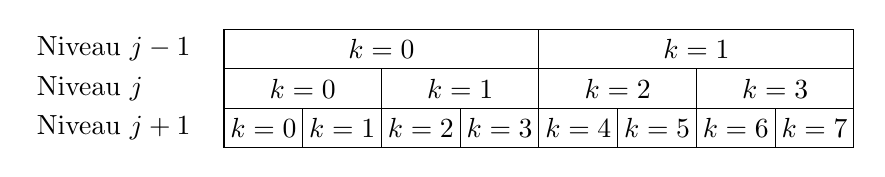
\begin{tikzpicture}


\node[anchor=west] at (-6.5, -.25) {Niveau $j+1$};
\node[anchor=west] at (-6.5, .25) {Niveau $j$};
\node[anchor=west] at (-6.5, .75) {Niveau $j-1$};
% Niveau j-1

\draw (-4,.5) rectangle (0,1);
\draw (0,.5) rectangle (4,1);

    % Niveau j
\draw (-4,0) rectangle (-2,.5);
\draw (-2,0) rectangle (0,.5);
\draw (0,0) rectangle (2,.5);
\draw (2,0) rectangle (4,.5);
%\node at (1,1.75) {$k=2$};

% Niveau j+1

\draw (-4,-.5) rectangle (-3,0);
\draw (-3,-.5) rectangle (-2,0);
\draw (-2,-.5) rectangle (-1,0);
\draw (-1,-.5) rectangle (0,0);
\draw (0,-.5) rectangle (1,0);
\draw (1,-.5) rectangle (2,0);
\draw (2,-.5) rectangle (3,0);
\draw (3,-.5) rectangle (4,0);

% Relations
\node at (-2, .75) {$k=0$};
\node at (+2, .75) {$k=1$};

\node at (-3, .25) {$k=0$};
\node at (-1, .25) {$k=1$};
\node at (+1, .25) {$k=2$};
\node at (+3, .25) {$k=3$};

\node at (-3.5, -.25) {$k=0$};
\node at (-2.5, -.25) {$k=1$};
\node at (-1.5, -.25) {$k=2$};
\node at (-0.5, -.25) {$k=3$};

\node at (+0.5, -.25) {$k=4$};
\node at (+1.5, -.25) {$k=5$};
\node at (+2.5, -.25) {$k=6$};
\node at (+3.5, -.25) {$k=7$};


\end{tikzpicture}
\caption{Exemple de grille dyadique}
\label{fig:schema_sdyadique}
\end{figure}
%         Dans ce qui suit il est supposé sans perte de généralité que la discrétisation se fait sur l'intervalle $[0,1]$,
%         ainsi le niveau $j$ correspond à des cellules de tailles $1/{2^j}$ et la cellule $k$ du niveau $j$ est centrée en
%         $x_k^j = \frac{k+(k+1)}{2} \frac{1}{2^j} = \frac{2k+1}{2^j}.$
%         La notion d'ondelette se définit de la manière suivante:
%         \begin{definition}[Ondelette]
%             Une ondelette est une fonction $\Phi \in L^2(\mathbb R)$ à support compact de moyenne nulle \cite{MallatWaveletTourChap4}.
%         \end{definition}
%         Cette fonction permet de définir un ensemble de fonctions :
%             $$\mathcal{B}= \left\{\Phi_{j,k} : x \mapsto \Phi(2^j x - k)\;\middle|\;(j,k) \in \{1, \dots, J\} \times \{0, \dots, 2^j - 1\}\right\}$$
%         Chaque $\Phi_{j,k}$ correspond à l'ondelette de base $\Phi$, mise à l'échelle des cellules du niveau $j$ et translatée pour être centrée sur la cellule $k$.
%         Alors la transformée en ondelette discrète peut être définie comme une projection de $L^2(\mathbb R)$ dans $\mathrm{Vect}(\mathcal{B})$
%         \begin{definition}[Transformée en ondelette discrète - \textit{Discrete Wavelet Transform, DWT}] 
%             La transformée en ondelette de $f \in L^2$ est sa projection dans $\mathrm{Vect}(\mathcal{B})$ : 
%             Le coefficient $\gamma_k^j$ de sa DWT sur la cellule $k$ au niveau de résolution $j$ est:
%             \begin{align}
%                 &\gamma_k^j =  \frac{1}{N_j} \left< f \vert \Phi_{i,j} \right>  = \frac{1}{N_j} \int_\mathbb{R} \Phi(2^j\cdot k - t)f(t) \text{d} t,\\\notag
%                 &\text{Où $N_j$ est un coefficient normalisation dépendant du niveau $j$.}
%             \end{align}
%             Contrairement à une transformée de Fourier, les coefficients ne dépendent pas d'une mais de deux variables. En effet, 
%             la transformée en ondelette est plus riche d'informations. Là où la transformée de Fourier ne donne qu'une information 
%             sur le contenu fréquentiel d'un signal, la transformée en ondelette donne une information sur le contenu en fréquence \underline{et}
%             sur la localisation de ce contenu fréquentiel.
%         \end{definition}

%     \subsubsection{La notion de détails}
%         La multi-résolution adaptative se sert de la transformée multi-échelle pour adapter le maillage, c'est à dire compresser l'information (voir \ref{par:adaptation}).
%         Cela requiert l'introduction de la notion de détail. Ce concept permet de ne pas utiliser la transformée en ondelette pour quantifier le contenu absolu porté par une échelle particulière,
%         mais plutôt à comprendre en quoi ce contenu s'éloigne de ce que les échelles supérieures pourraient laisser supposer, en quoi il est \textit{inattendu}.
%         Pour résumer à partir d'un niveau de résolution $j$, on définit un \textbf{prédicteur} polynomial, qui tente d'inférer l'allure de la fonction au niveau $j+1$.
%         Puis le \textbf{détail} ne cherche pas naïvement à quantifier et localiser l'information contenue aux échelles du niveau $j+1$ mais plutôt, 
%         à quantifier l'écart à la prédiction polynomiale.
%         \paragraph{Le prédicteur}
%             Donné un point central $(x_0,y_0)$, et $2s$ voisins $(x_{-s},y_{-s}),(x_{-s+1},y_{-s+1})\dots (x_{s-1},y_{s-1}),(x_s,y_s)$, un prédicteur polynomial 
%             ponctuel cherche le polynôme $P$ de degré $2s$ passant par ces $2s+1$ points. Cela permet d'inférer des valeurs pour $y$ en tout point $x$.
%             Pour trouver $P(X) = \sum_{k=0}^{2s} a_k X^k$ revient à résoudre le système linéaire:
%             \begin{align}
%                 \forall j \in \{-s,\dots 0 ,\dots,s\}: y_j = \sum_{k=0}^{2s} a_k x_j^k
%             \end{align}
%             Ce stage se focalise sur les volumes finis, donc ce n'est pas un prédicteur ponctuel, adapté au différences finies (voir \ref{def:vol_finis}), qui est utilisé mais un prédicteur sur la valeur moyenne. 
%             Il ne cherche à imposer les valeurs en chaque point mais à fixer la valeurs moyenne sur chaque cellule,
%             cela ajoute peu de complexité puisqu'il suffit d'ajouter une intégration lors de l'établissement du système linéaire pour travailler sur les valeurs moyennes.
%             Pour l'usage que souhaité ici, il s'agit en d'évaluer la solution sur la cellule $k$ du niveau de résolution $j$ 
%             (ce qui correspond à la cellule de centre $x_k^j = (k+1/2) 2^{-j}$) au niveau de résolution supérieure $j+1$,
%             il faut donc appliquer le correcteur linéaire centré sur $x_k^j$ en $x_{\pm} = \pm 2^{-(j+1)}$. En pratique cela revient à faire une combinaison linéaire des $2s$ voisins
%             qui vient corriger la valeur en $x_k^j$.
%             Le prédicteur dépend donc du nombre de voisins pris de part et d'autre, ce nombre noté $s$ et appelé le \textit{stencil} du prédicteur.
%             Plus $s$ est grand plus l'opération de prédiction est précise (mais peut éventuellement devenir bruitée\footnote{Ce n'est pas détaillé ici mais le lecteur se réfèrera à la théorie de l'interpollation...})
%             et plus elle est coûteuse. Le coût exact n'est pas évident à estimer puisque qu'une combinaison linéaire
%             quelques termes se fait en $O(1)$ sur les machines modernes, toutefois quelques subtilités détaillé en \ref{par:adaptation} interviennent.
%             Ainsi les valeurs usuelles tu stencil sont généralement $s=1$ ou $s=2$

%         \paragraph{Les détails}
%             À présent que le prédicteur à été décrit le concept de détail peut enfin être abordé. On suppose que l'on dispose d'une fonction $\tilde u^j$
%             qui soit une approximation de la fonction $u$, au niveau de résolution $j$. Comme vu précédemment, le prédicteur permet d'obtenir une approximation 
%             de $u$ au niveau $j+1$ grâce à $\tilde u^j$. Cette prédiction est noté $\hat u^{j+1}$. Les détails à la résolution $j+1$ sont alors définis comme les 
%             coefficient de la transformée multi-échelle de la différence entre cette prédiction et la vraie fonction: $u-\hat u^{j+1}$.
%             Alors les coefficients de détails n'encode que ce qui n'était pas prédictible par l'interpolateur polynomial. 
%             Ce concept de détail est essentiel. 
%             En pratique on ne réalise pas l'opération comme expliqué plus haut puisque à prédicteur et ondelette fixés $\Phi$, il existe une \textit{ondelette duale} $\Psi$
%             qui permet directement d'obtenir les détails pour la DWT sur $\Phi$ en réalisant une DWT sur $\Psi$ ce qui accélère considérablement les calculs.\par
%             % Une autre façon de voir la notion de détail est la suivante:
%             % pour un niveau de résolution $j$ on note $V_j = \text{Vect}\Bigl((\Phi_k^j)_k\Bigr)$, c'est à dire l'ensemble de fonction 
%             % représentables par les ondelettes de niveau $j$.
%             % Pour les ondelettes classiques\footnote{C'est en tout cas vrai pour les ondelettes de Haar\cite{postePoly}.} la relation suivante est vérifiée
%             % $V_0 \subset V_1 \subset V_2 \subset \ldots \subset V_N$. Et bien alors l'espace des détails, celui accessible par l'ondelette duale est $Q_{j+1}$
%             % le supplémentaire de $V_j$ dans $V_{j+1}$, en d'autre terme, il représente toutes les informations, les \textit{détails} contenues dans 
%             % le niveau d'approximation $V_{j+1}$ qui n'étaient pas prise en compte par $V_j$ (à l'échelle $j$ ce n'était que des détails). 
%             % Les coefficients de la décomposition par l'ondelette duale sont  Ainsi grâce à l'ondelette duale, 
%             % il est possible de calculer les coefficients de détails $d_k^j$ qui à chaque montée en résolution n'encode que l'information qui n'était 
%             % pas contenue dans la décomposition en ondelette au niveau précédent.\par
%             % Les deux visions ne sont pas rigoureusement les mêmes, la première représente ce qui est réalisé en pratique lors de la MRA, la seconde 
%             % est la vision standard de la théorie des ondelettes. Toutefois les deux approches ont la même motivation, ne calculer et ne mettre en valeur à chaque
%             % niveau que ce qui est nouveau, ce qui n'était pas contenu dans les niveaux précédents.
        
%         \paragraph{Intuition sur les détails}
%             Lorsque l'on s'intéresse aux coefficients de détails $d_k^j$,
%             l'indice $j$ de \textit{dilatation} fixe l'échelle analysée, c'est à dire la longueur d'onde analysée. Par exemple si $j=5$, 
%             les coefficients $d^5_k$ donne une information sur l'information portée par les longueurs d'onde de l'ordre de $2^{-5} = 1/32$.
%             La variable $k$ précise l'indice de la cellule analysée.
%             Par exemple $\Vert d^5_10 \Vert > \Vert d^5_5 \Vert$ signifie que l'information portée par l'échelle $1/32$
%             est plus importante au voisinage de la case $10$ qu'au voisinage de la case $5$.
%             De même si $\Vert d^j_7 \Vert > \Vert d^{j+1}_{14} \Vert$ cela signifie qu'au voisinage de $x=\frac{7}{2^j}$
%             les longueurs d'ondes $\frac{1}{2^j}$ sont plus présentes que les longueurs d'ondes $\frac{1}{2^{j+1}}.$
%             Pour se fixer les idées, c'est comme si la transformée de Fourrier n'avait qu'une vision globale du contenu en fréquence, 
%             quelle ne voyait que la moyenne sur le domaine de la transformée en ondelette pour chaque longueur d'onde.
%             \begin{align}
%                 \Vert TF\bigl[ f \bigr](\omega = 2^j) \Vert^2 \sim \Vert \sum_{k} d^j_k \Vert^2.
%             \end{align}
%             \par 
%             Grâce à cette notion de détaille la décomposition multi-échelle permet une description de la solution physique où l'apport à la solution de chaque échelle,
%             de chaque distance typique est quantifié, les coefficients $d_k^j$ décrivant l'information contenue dans les échelles de l'ordre de $2^{-j}$.
% \subsection{L'adaptation}\label{par:adaptation}
%     \subsubsection{La compression par décomposition multi-échelle}
%             Pour compresser une fonction (ou une image comme dans le processus \texttt{jpg}), le processus est très simple, il suffit de fixer un seuil de compression $\varepsilon > 0$,
%             de calculer les coefficients de détails de la fonction, 
%             puis d'omettre (en pratique de retirer de la mémoire) les coefficient dont la norme est inférieure à $\varepsilon$.
%             En pratique le coefficient de compression dépend du niveau étudié puisque le volume des cellules mise en jeu chute avec le niveau $j$
%             (un détail de $10^{-2}$ à moins d'importance s'il porte sur des cellules de taille $10$ que sur des cellules de taille $10^{-5}$).
%             En pratique l'algorithme serait le suivant:
%             \begin{enumerate}  
%                 \item Calculer les coefficients $d_k^j$.
%                 \item Pour chaque niveau $j$ et chaque coefficient $d_k^j$: Si $\vert d_k^j \vert < \varepsilon_j = 2^{-j}\varepsilon$, alors $d_k^j\leftarrow 0$, les coefficients sont seuillés.
%                 \item[] Pour reconstruire au niveau de résolution souhaité: utiliser les détails jusqu'au niveau $j$ le plus fin conservé puis utiliser le prédicteur 
%                 pour interpoler jusqu'au niveau désiré. Le vocabulaire est heureusement choisit, pour compresser on omet les détails négligeables l'on conserve les détails importants.
%             \end{enumerate}
%     \subsubsection{L'adaptation de maillage et l'heuristique d'Harten}
%             L'adaptation de maillage, est une variation de la compression par décomposition multi-échelles précédemment décrite. 
%             C'est est une opération de compression de solutions physiques \textit{prudente}.
%             Les coefficients y sont seuillés de manière moins impitoyable: certains coefficients qui devraient être écartés
%             par la compression sont malgré tout préservés. Ce choix se fait sur la base d'intuitions physiques, 
%             la plus connue étant \textit{l'heuristique d'Harten}, introduite par Ami Harten \cite{harten1994}, le père de la MRA.
%             Elle stipule que même si un coefficient de détail $d_k^j$ devrait être supprimé, si le niveau de détail du niveau supérieur 
%             (c'est à dire $d^{j-1}_{\lfloor k/2 \rfloor}$) est particulièrement élevé, par exemple qu'il est par deux fois supérieur au seuil $\varepsilon_{j-1}$,
%             alors le coefficient doit être conservé. En d'autre terme, même si la compression considère l'information à l'échelle $j$ négligeable,
%             l'intuition physique pose son véto puisque les échelles supérieurs sont de grandes magnitudes et que cela présage que dans 
%             les pas de temps a venir les échelles seront nécessaires à la fidèle capture des phénomènes physiques simulés. Par exemple cela peut signifier qu'un front
%             d'onde est en train d'arriver dans les zone étudiée, il faut donc que la simulation puisse en capter toute la richesse.
% \subsection{Algorithmes de simulation numérique}
%     \subsubsection{Algorithme général}
%             L'intégration de la MRA un algorithme de simulation physique se fait de la manière suivante: 
%             tous les $n_{MRA}$ pas de temps (éventuellement être à chaque pas de temps), 
%             la solution physique est adaptée selon le procédé explicité ci-dessus. Les détails précédemment omis
%             devenant nécessaires sont obtenus grâce au prédicteur. Puis la simulation se poursuite à partir de cette grille de calcul adapté.
%             L'économie de mémoire se fait puisque tous les détails ne sont pas stockés et l'économie de calculs puisque moins de cellules sont mises en 
%             jeu lors du déroulement de l'algorithme de simulation.\par
%             Par exemple, en dimension une, si une zone est adapté avec un niveau de détail de niveau 5, la densité de cellule sur lequel il faut réaliser des est de $2^5$
%             et la densité mémoire est de $\sum_{j=0}^5 2^j$. Si le niveau le plus fin de la grille est par exemple 9, il y a un gain computationnel théorique de l'ordre de 
%             $2^{9-5}=16$ et en terme de mémoire une économie de l'ordre de $\frac{\sum_{j=0}^5}{2^8} > 10$. Ce gain est exponentiel avec la dimension du problème.
%     \subsubsection{Le cas volumes finis}
%             Il faut détailler ce qui signifie dans le cadre des volumes finis, \textit{poursuivre la simulation sur la grille de calcul adaptée}.
%             Le maillage adapté est constitué de cellules de tailles différents.
%             Il s'agit alors pour chacune de ces cellules de prédire la valeur moyenne en son sein au pas de temps suivant, c'est à dire faire évoluer le maillage.
%             Cela se fait en évaluant un flux à partir des valeurs de la solution aux interfaces de la cellule. 
%             Tout l'objet des volumes finis est: à partir de valeurs moyennes sur les cellules voisines, estimer les valeurs ponctuelles aux interfaces. 
%             La MRA amène alors une subtilité, les schémas volume finis usuels s'appuient sur des cellules de volumes similaires de l'ordre de $\Delta x^d$.
%             L'approche usuelle en MRA, est dite \emph{sans reconstruction des flux}. Ainsi les cellules utilisées pour évaluer les flux numériques sont celles 
%             du maillage adapté, c'est à dire celles au niveau que la multirésolution a conservé. Une approche moins standard est de reconstruire 
%             les cellules nécessaires à l'évaluation des flux au niveau le plus fin. Ainsi la méthode est quand même adaptée, 
%             il y a moins de flux à reconstruire puisque la solution est adaptée, mais les valeurs nécessaire à leur évaluations sont reconstruites.
%             Cette approche est potentiellement plus précise et est peut-être un bon compris entre coût calcul et précision.


%     \subsubsection{Le débat sur la reconstruction}
% \subsection{Impact sur les solutions}
%     \subsubsection{}
%     \subsubsection{}
% \subsection{Implémentations de la multi-résolution}
%     \subsubsection{Méthodes usuelles}
%             \paragraph{Les approches \textit{patch-based}}
%             \paragraph{Les approches \textit{cell-based}}
%     \subsubsection{Le logiciel Samurai}
%             \paragraph{Un tructure de données originale}